\subsection{Primer Prototipo}
Con el fin de poder familiarizarse con el motor de juego Unity
se desarrollo un primer prototipo. Este primer prototipo basa su funcionamiento 
en algunas de las mecánicas de la sección de plataformas del segundo nivel, con 
algunas diferencias en cuanto al manejo de la cantidad de vida, el personaje 
jugable y la colocación de algunos botones en la GUI del juego.
\\
\par
En el primer prototipo el jugador puede:
\begin{itemize}
	\item Mover al persoanje jugable hacia la derecha.
	\item Mover al personaje jugable hacia la izquierda.
	\item Hacer que el personaje jugable salte.
	\item Hacer que el personaje jugable dispare.
\end{itemize}

Con este primer prototipo el equipo de desarrollo se familiarizó con:
\begin{itemize}
	\item Crear Sprites.
	\item Implementar un personaje jugable.
	\item Implementar Interfaz gráfica.
	\item Manejar un marcador para el juego.
	\item Manejar efectos especiales para determinadas acciones del personaje jugable.
	\item Manejar archivos para preservar datos de la partida.
	\item Crear una inteligencia artificial sencilla para los enemigos.
\end{itemize}

\subsubsection{Creando sprites.}
Los sprites, dentro de unity, son todos aquellos objetos gráficos de dos 
dimensiones. Para este prototipo en particular se crearon sprites haciendo uso 
de Corel Draw X5\copyright y Adove Photoshop\copyright ; y también se descargaron 
algunos sprites desde el sitio web GameArt2D.  

\subsubsection{Implementación del personaje jugable}
Para la implementación del personaje jugable se creo un GameObject a partir de 
un Sprite. Y posteriormente se agregaron los componentes: RigidBody2D, para el 
manejo de físicas y movimiento; BoxCollider2D, para la detección de colisiones; 
Animator, para vincular la maquina de estados de las animaciones; y la clase PlayerManager, clase equivalente a la clase Player descrita en el apartado 
\ref{ClasesJuego}. En la figura \ref{figPersonajeJuCom} se puede observar la 
configuración de los componenetes RigidBody2d, BoxCollider2D y Animator.

\begin{figure}
  \centering
   \subfigure[Configuracion del componente Animator (Autoría propia).] {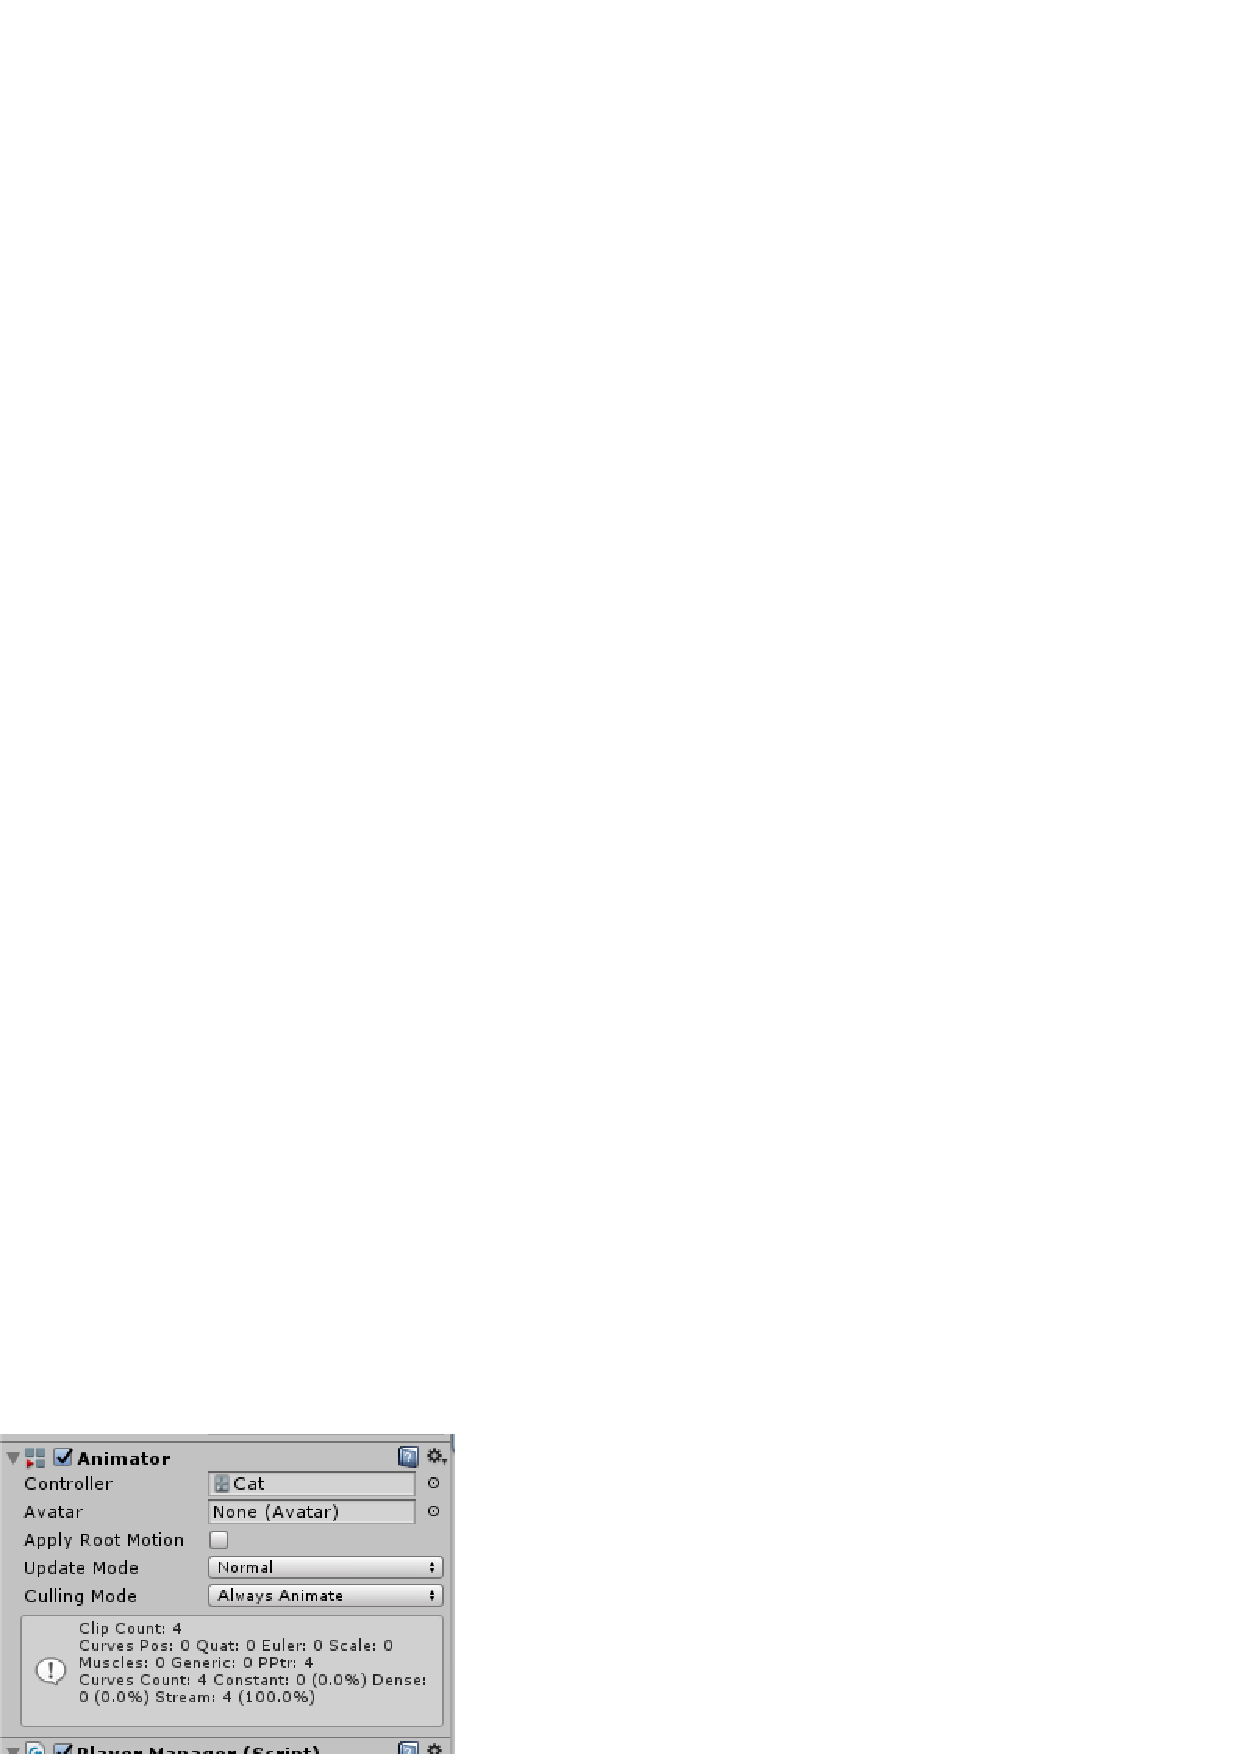
\includegraphics[width=0.3 \textwidth]{05TrabajoRealizado/03Unity/imagenes/02AnimatorGAtos}}
   
 	\subfigure[Configuracion del componente BoxCollider2D (Autoría propia).] {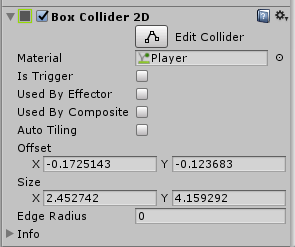
\includegraphics[width=0.3 \textwidth]{05TrabajoRealizado/03Unity/imagenes/02BoxColiderGAtos}}
 	
\subfigure[Configuracion del componente RigidBody2D (Autoría propia).] {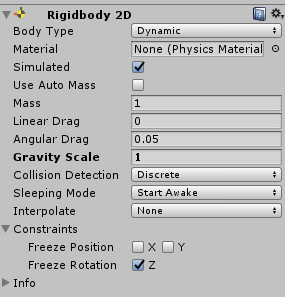
\includegraphics[width=0.3 \textwidth]{05TrabajoRealizado/03Unity/imagenes/02RigidBGAtos}}
  \caption{Componentes del Personaje jugable.}
  \label{figPersonajeJuCom}
\end{figure} 

Las animaciones del personaje jugable se gestionaron a través de una maquina de 
estados (ver figura \ref{figMaqEsCat}). Las transiciones de la maquina de 
estados son controladas por la clase PlayerManager, quien se vale del componente 
Animator para hacer dichas transiciones.

\begin{figure}
  \centering
   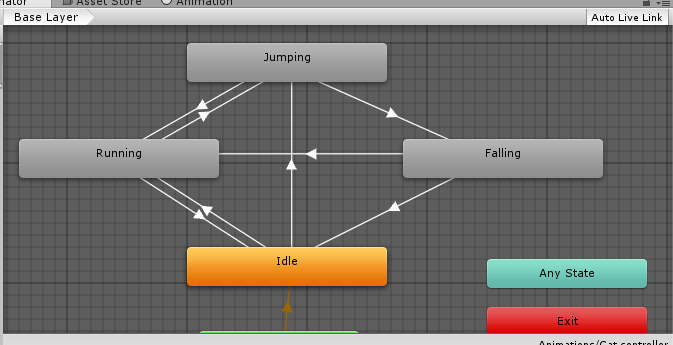
\includegraphics[width=0.6 \textwidth]{05TrabajoRealizado/03Unity/imagenes/02AnimacionGato}
  \caption{Maquina de estados del personaje jugable del prototipo 1 (Autoría propia).}
  \label{figMaqEsCat}
\end{figure} 

PlayerManager contiene casi los mismos tributos y métodos que la clase Player. 
Pero, es importante recalcar que PlayerManager no dispone de los atributos 
correspondientes a la cantidad de vida disponible ni a la cantidad de 
\textit{Tonalli}. Una de las diferencias más significativas entre ambas clases es que 
PlayerManager instancía en algunos de sus métodos clases de tipo controlador 
para utilizar métodos de estas clases (Ver figura \ref{figInstanciaCtrl}), 
mientras que la clase Player respeta la jerarquía de clases y al ser una clase de 
tipo actora no puede modificar a un controlador. En cuanto a la funcionalidad que 
tienen en común; al igual que la clase Player, PlayerManager permite al personaje jugable desplazarse de manera horizontal, saltar y disparar. Para garantizar que el método de Fire funcione, fue necesario crear un GameObject para el disparo. A éste 
GameObject se le agregaron los componentes: RigidBody2D, para el control de fisicas 
y movimiento; CircleCollider2D, para la detección de colisiones; y dos clases BulletCtrl 
y DestroyWithDelay.
\\
\par
 
\begin{figure}
  \centering
   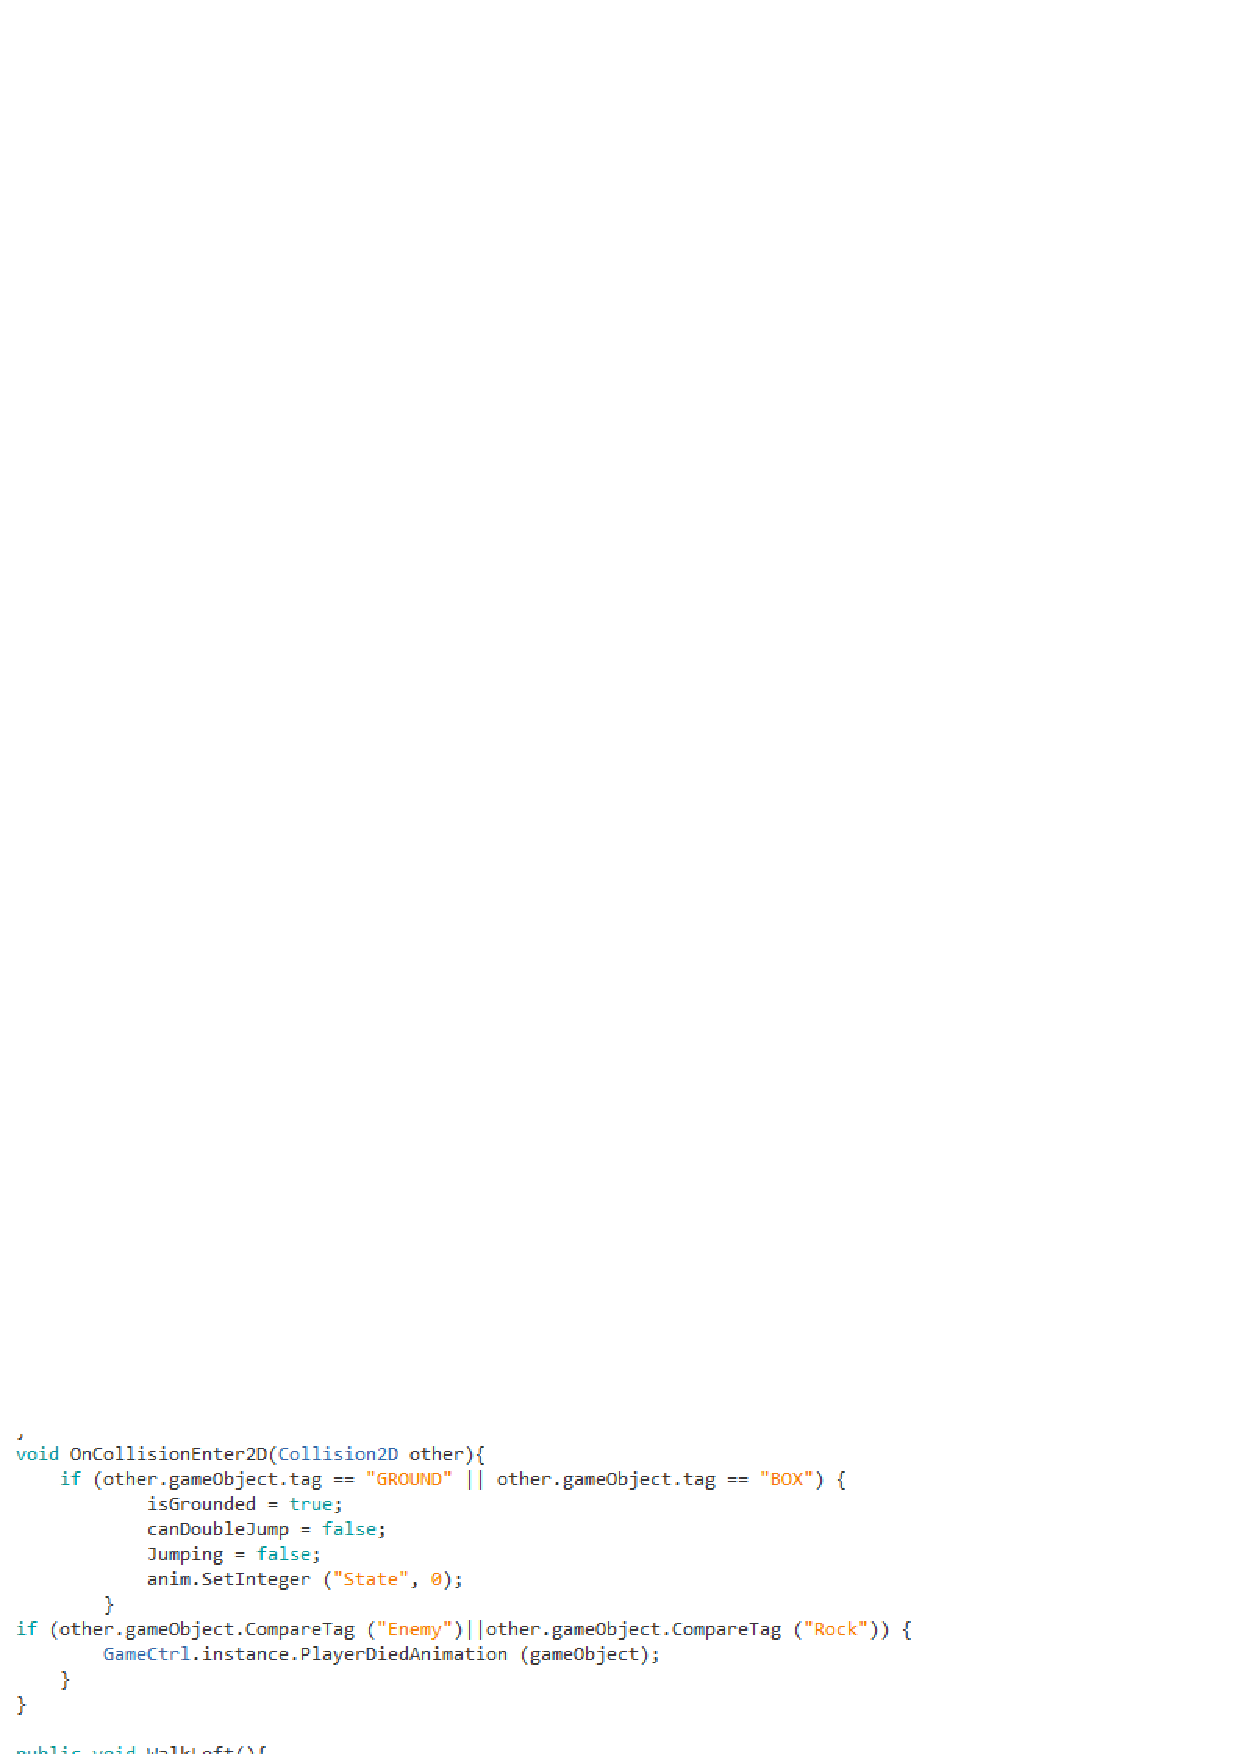
\includegraphics[width=0.6 \textwidth]{05TrabajoRealizado/03Unity/imagenes/02GatoCtrl}
  \caption{PlayerManager instancia clase de tipo controlador para actualizar marcadores (Autoría propia)}
  \label{figInstanciaCtrl}
\end{figure} 


En cuanto a la detección y respuesta de colisiones, la clase PlayerManager se 
vale de la capacidad de Unity para etiquetar objetos. Bajo este sistema de 
etiquetación se puede determinar una respuesta en concreto a todos los objetos 
que colisionen con el personaje jugable y que compartan una misma etiqueta. A 
continuacion se listan algunas de la etiquetas que se manejaron en este prototipo, 
seguida de la respuesta del personaje jugable al colisionar con un 
objeto bajo esta etiqueta:
\begin{itemize}
	\item \item Ground: PlayerManager actualiza atributos que habilitan la capacidad 
	de usar el método Jump y de que estado de animación activar cuando el personaje 
	jugable se mueva.
	\item Enemy: PlayerManager instancía la clase GameCtrl y le pide que ejecute el 
	método PlayerDiedAnimation para indicar la muerte del personaje jugable (ver 
	figura \ref{figPersonajeResEne}).
	\item Dog: PlayerManayer instancía la clase GameCtrl y le pide que ejecute el 
	método UpdateXoloCount, despues destruye el objeto con la etiqueta Dog 
	y en su posición muestra un efecto especial de brillos. 
\end{itemize} 

\begin{figure}
  \centering
  
   \subfigure[Personaje Jugable antes de colisión con enemigo (Autoría propia).] {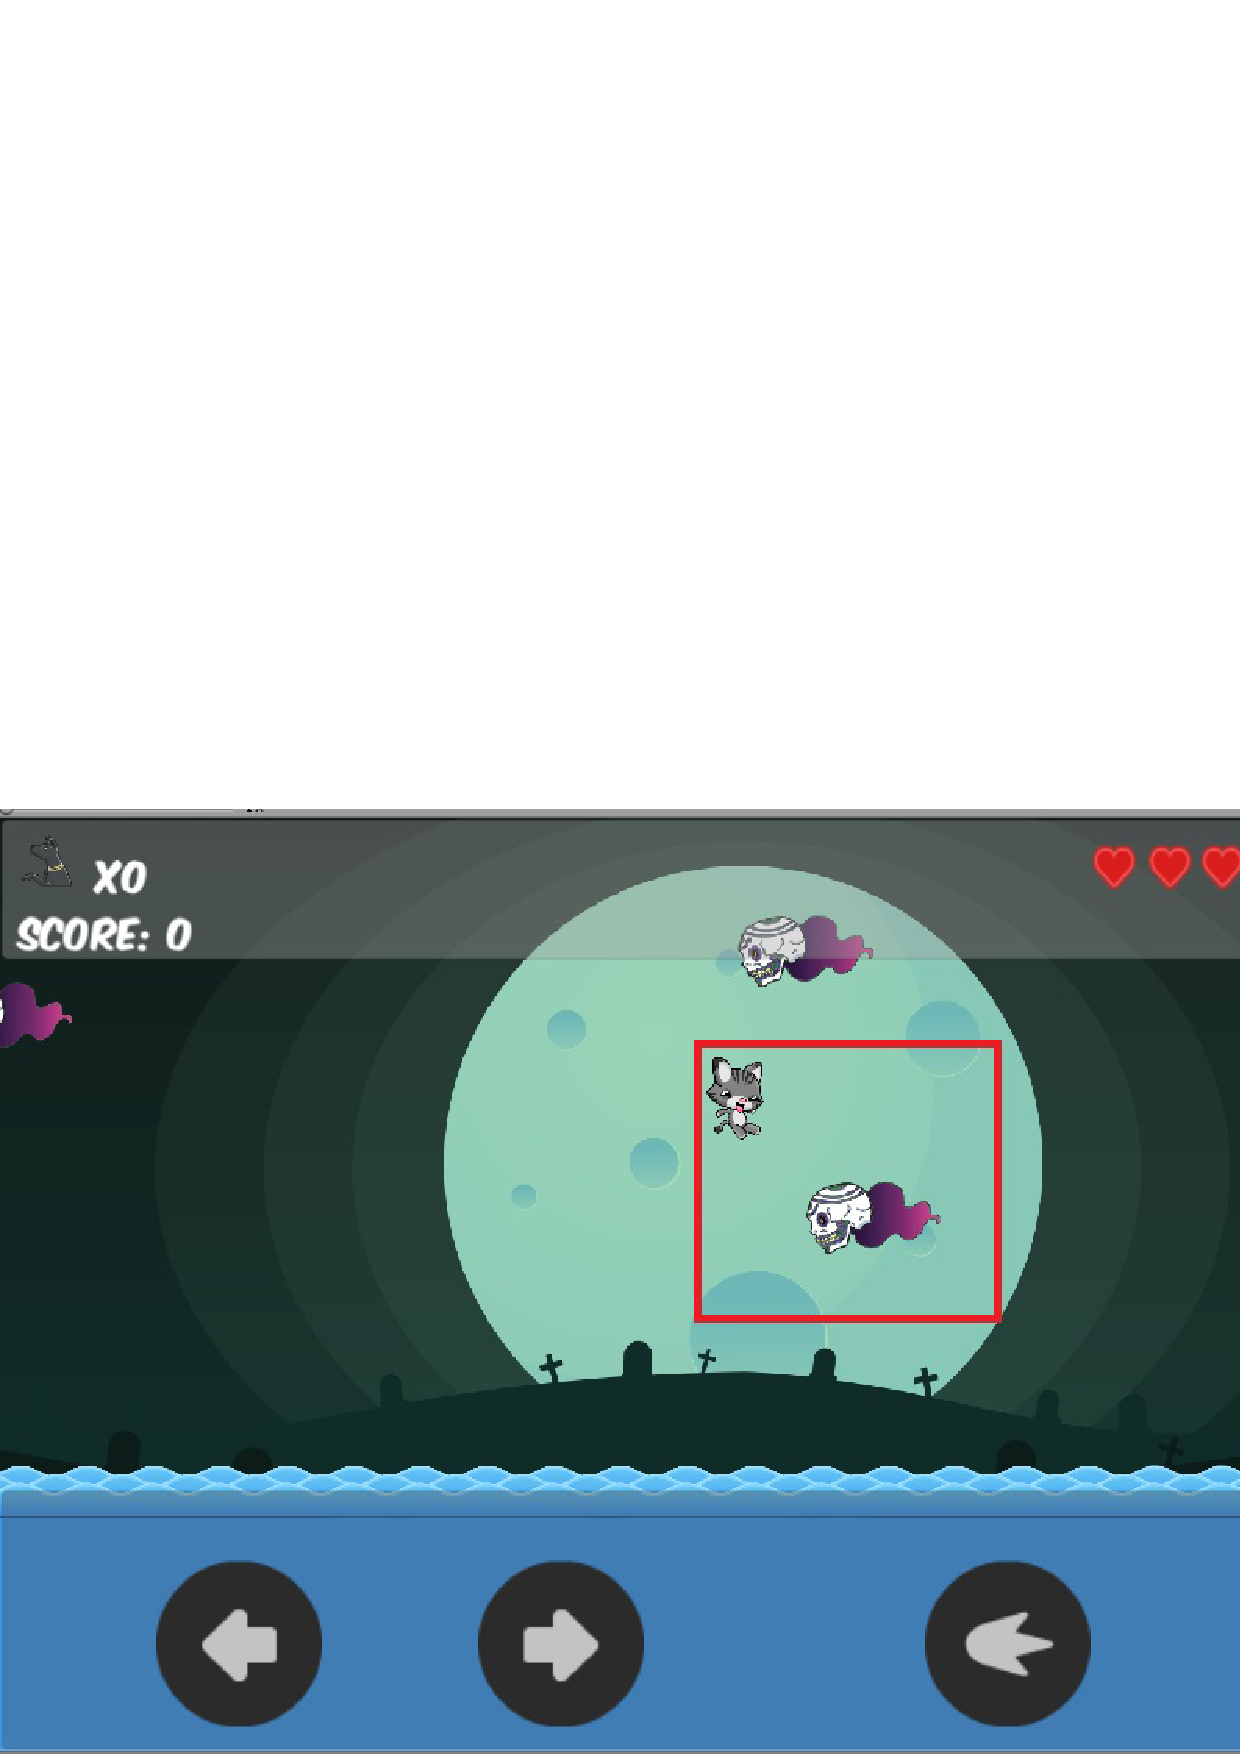
\includegraphics[width=0.4 \textwidth]{05TrabajoRealizado/03Unity/imagenes/02reaccionColisionEnemi01}}
   
 	\subfigure[Ejecución del método PlayerDiedAnimation (Autoría propia).] {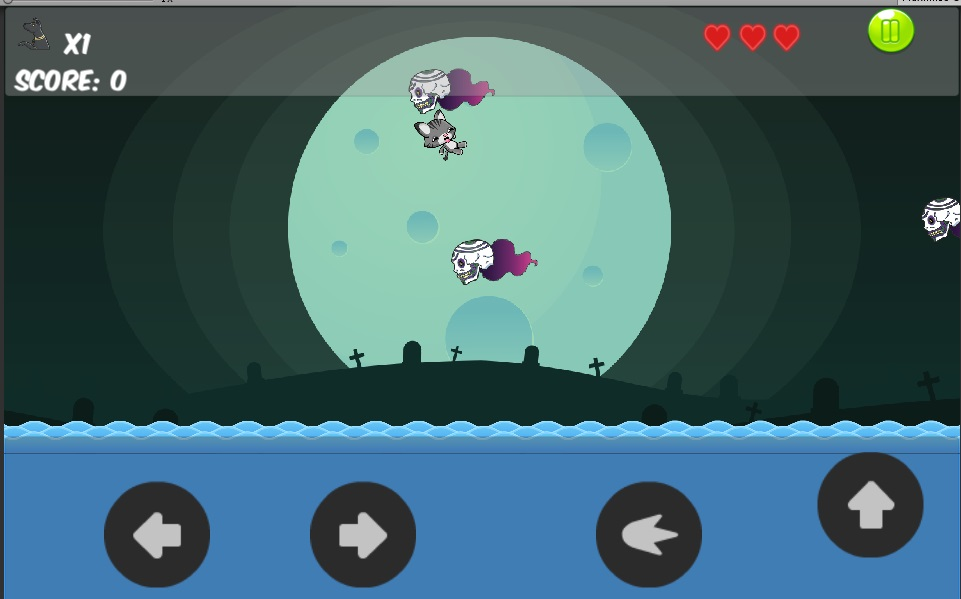
\includegraphics[width=0.4 \textwidth]{05TrabajoRealizado/03Unity/imagenes/02reaccionColisionEnemi02}}
 	
\subfigure[Actualización de la cantidad de vidas después de reiniciar el nivel tras colisión con el enemigo (Autoría propia).] {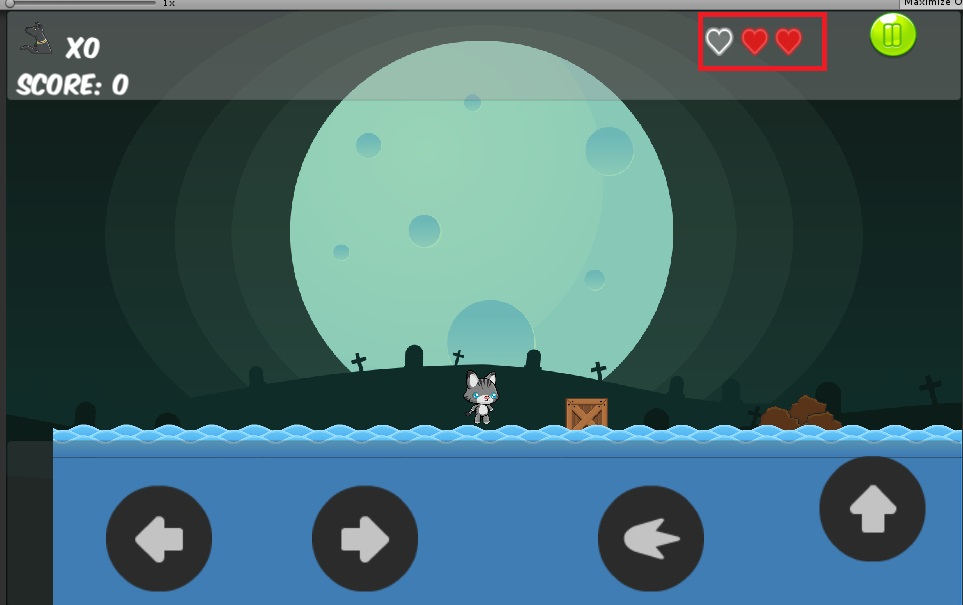
\includegraphics[width=0.4 \textwidth]{05TrabajoRealizado/03Unity/imagenes/02reaccionColisionEnemi03}}

  \caption{Respuesta visual del juego cuando el personaje jugable colisiona con un enemigo.}
  \label{figPersonajeResEne}
\end{figure} 

\begin{figure}
  \centering
  
   \subfigure[Personaje Jugable antes de colisión con xoloitzcuintle (Autoría propia).] {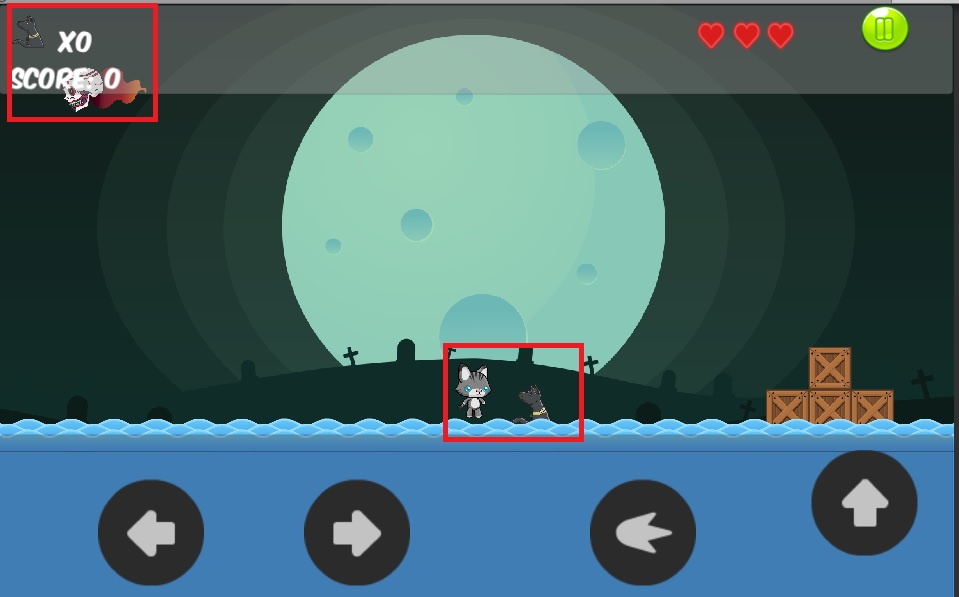
\includegraphics[width=0.4 \textwidth]{05TrabajoRealizado/03Unity/imagenes/02reaccionColisionperro01}}
   
 	\subfigure[Actualización del marcador de xoloitzcuintles (Autoría propia).] {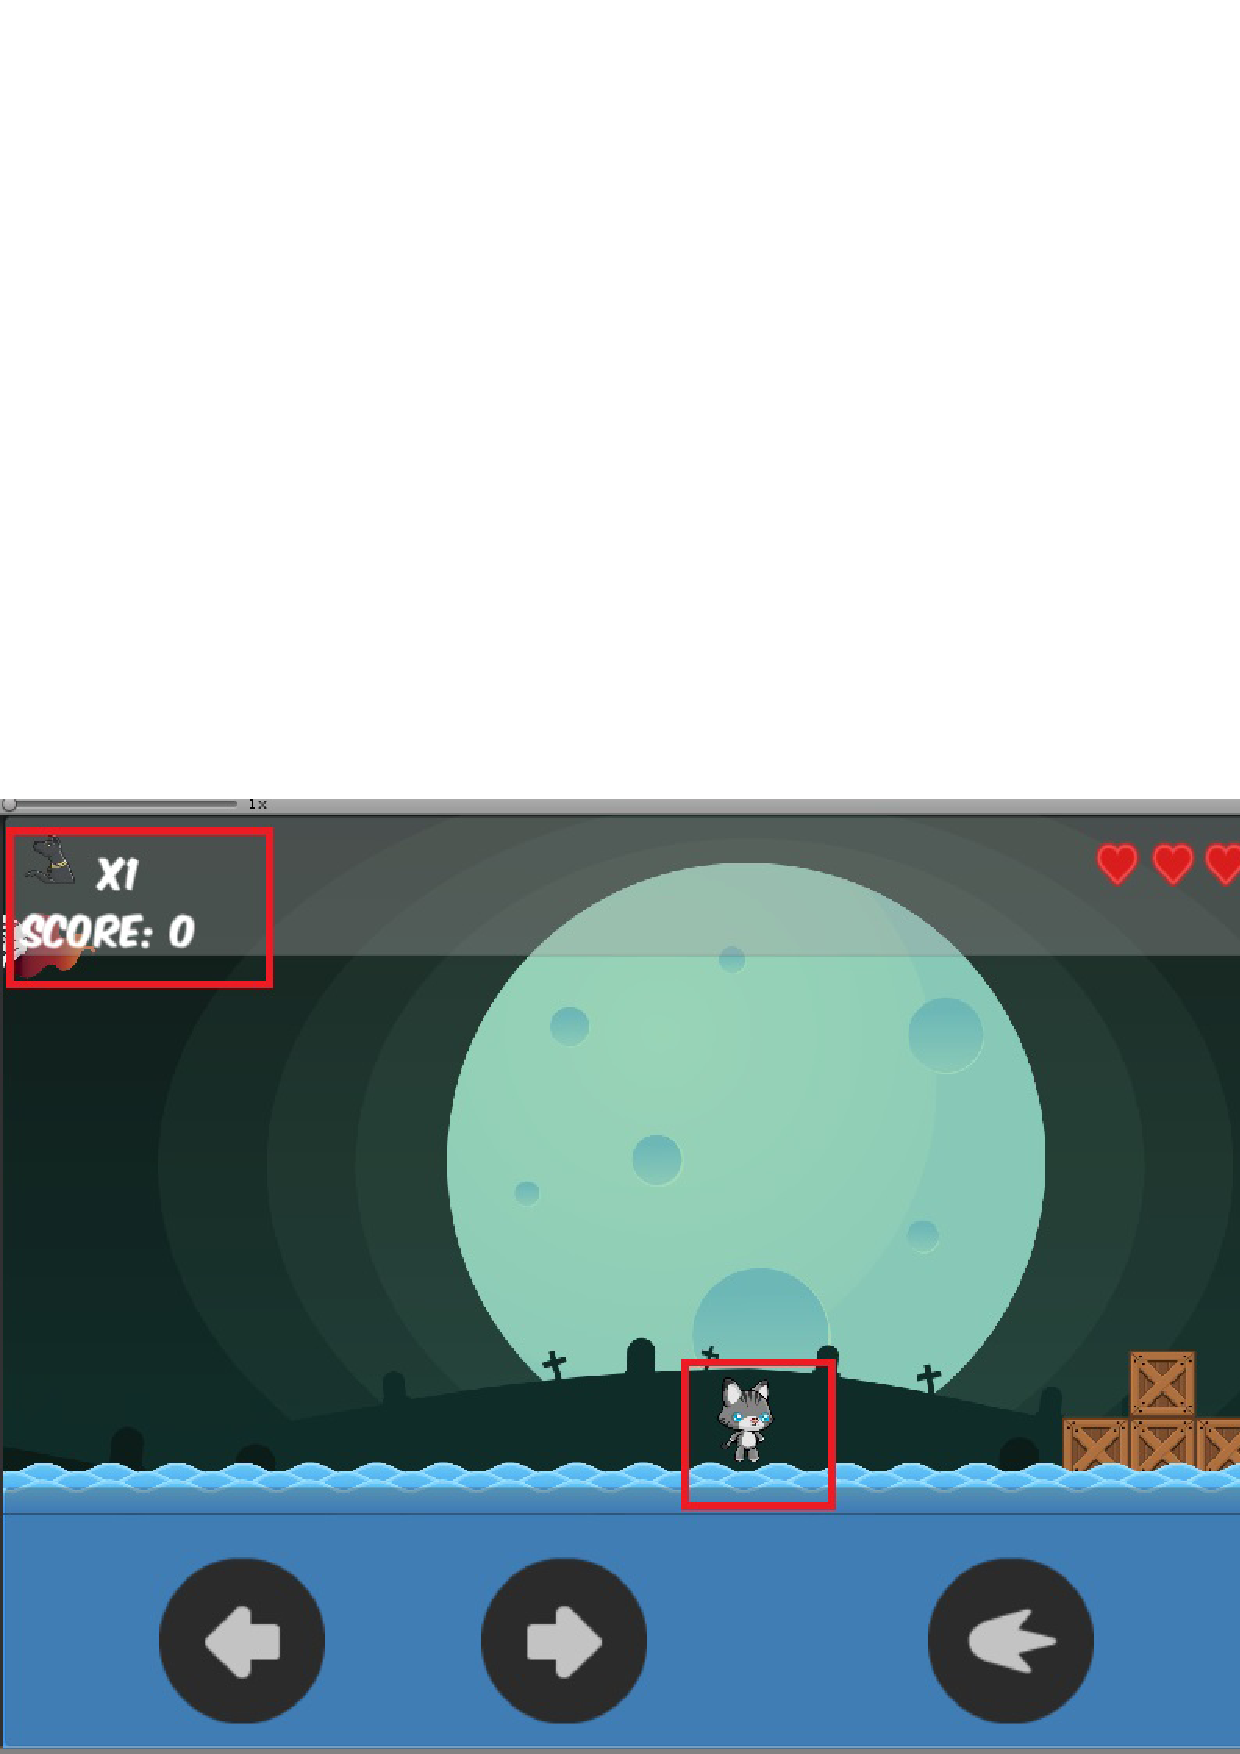
\includegraphics[width=0.4 \textwidth]{05TrabajoRealizado/03Unity/imagenes/02reaccionColisionperro02}}

  \caption{Respuesta visual del juego cuando el personaje jugable colisiona con un xoloitzcuintl.}
  \label{figPersonajeResXo}
\end{figure} 

\subsubsection{Implementar Interfaz gráfica} 
La interfaz gráfica se compone de dos canvas: uno para para los botones que 
controlan al juagdor y otro para mostrar los marcadores y numero de vidas del 
jugador (Ver figura \ref{figCanvas}).
\\
 \par
\begin{figure}
  \centering
   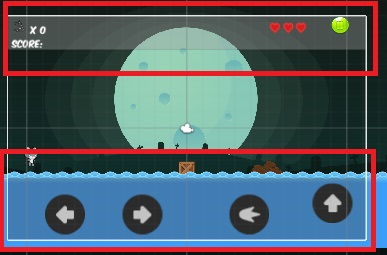
\includegraphics[width=0.4 \textwidth]{05TrabajoRealizado/03Unity/imagenes/02ConfiguracionCanvas02}
  \caption{La interfaz gráfica se divide en dos partes: 1. Canvas que muestra maracadores. 2. Canvas que contiene los botones que controlan al juagador(Autoría propia)}
  \label{figCanvas}
\end{figure} 

Ambos Canvas son configurados para que su tamaño se ajuste al objeto camara; de
 igual manera se configura su escalamiento para que su tamaño se adapte al de la
  pantalla que se tenga disponible evitando que los componentes del canvas 
  adquieran un tamaño que imposibilite el control del personaje jugable o la 
  visualización de información (ver figura \ref{figCanvasConf}).    
 \\
 \par
 \begin{figure}
  \centering
   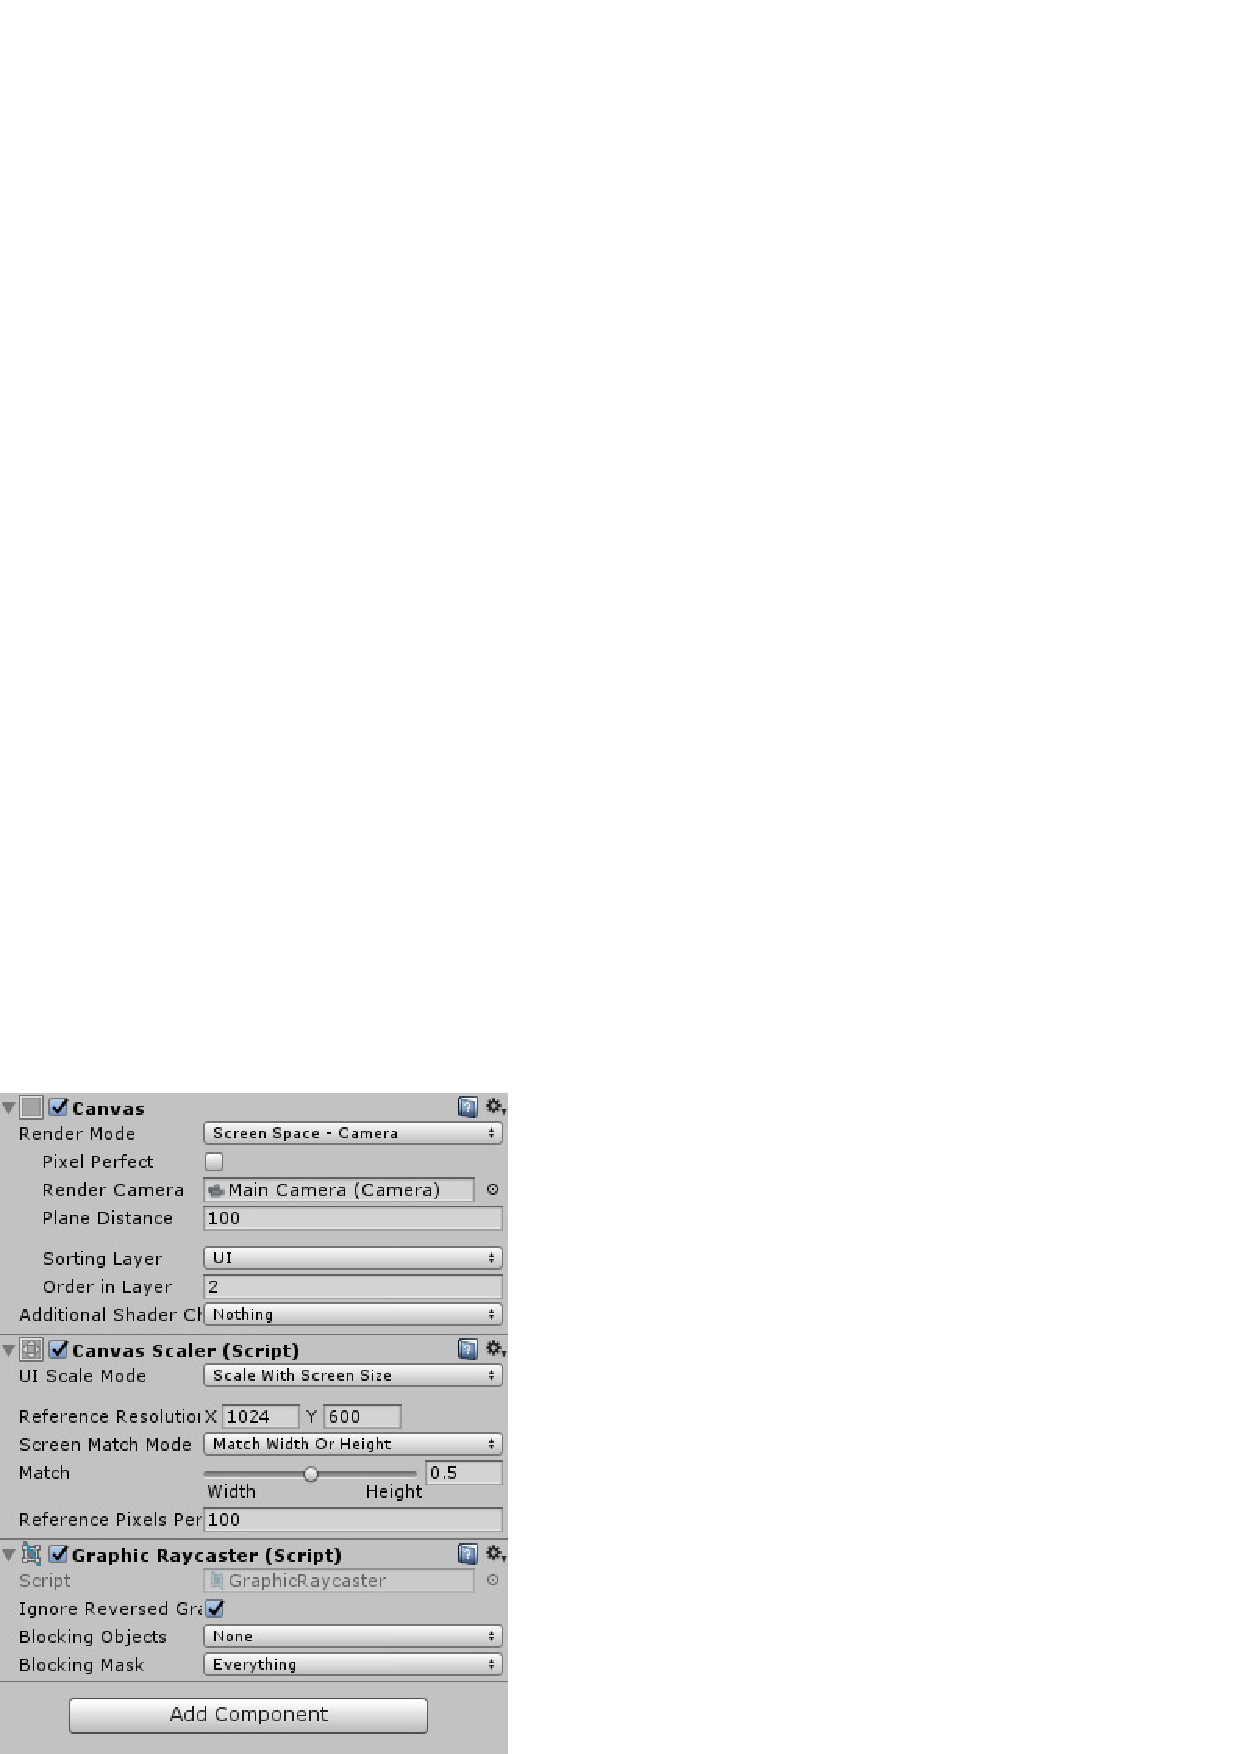
\includegraphics[width=0.4 \textwidth]{05TrabajoRealizado/03Unity/imagenes/02ConfiguracionCanvas}
  \caption{Configuración del canvas para que su tamaño sea el adecuado aun si el tamaño de pantalla cambia (Autoría propia)}
  \label{figCanvasConf}
\end{figure}
 El canvas que corresponde al conteo de vidas y al marcador es controlado por  
 la clase GameCtrl. Mientras que el canvas referente a los botones obtiene su  
 funcionalidad de la clase MobileUICtrl para comunicar al jugador con la clase 
 PlayerManager y con el personaje jugable.  
 
 \subsubsection{Manejo de un score para el juego y preservación de datos de la partida}
Como se mencionó con anterioridad, el marcador es controlado por la clase GameCtrl. 
Esta clase es el equivalente a la fusion de las clases LevelCtrl y DataFile 
descritas en el apartado \ref{ClasesJuego}. Al igual que como ocurre con Player 
y PlayerManager, GameCtrl y LevelCtrl y DataFile tienen métodos y atributos 
comunes. La diferencia más importante entre estas clases es que GameCtrl solo 
permite el almacenamiento de información para controlar un nivel y no puede 
gestionar la transición entre escenas. 
\\
\par
En cuanto al manejo del marcador, este se actualiza cada vez que el personaje jugable 
colisiona con un ojeto bajo la etiqueta Dog (ver figura \ref{figPersonajeResXo}) o el 
Jugador logra derrotar a un enemigo (ver figura ). En cada actualización del marcador, 
GameCtrl almacena los datos de la partida en un archivo de tipo binario. Cuando el 
personaje colisiona con un enemigo, GameCtrl permite mantener los valores de los 
maracadores y cantidad de vida del jugador, más no la posición que este tenía antes 
de la colisión.   
 
\begin{figure}
  \centering
  
   \subfigure[Personaje Jugable antes de disparar a enemigo (Autoría propia).] {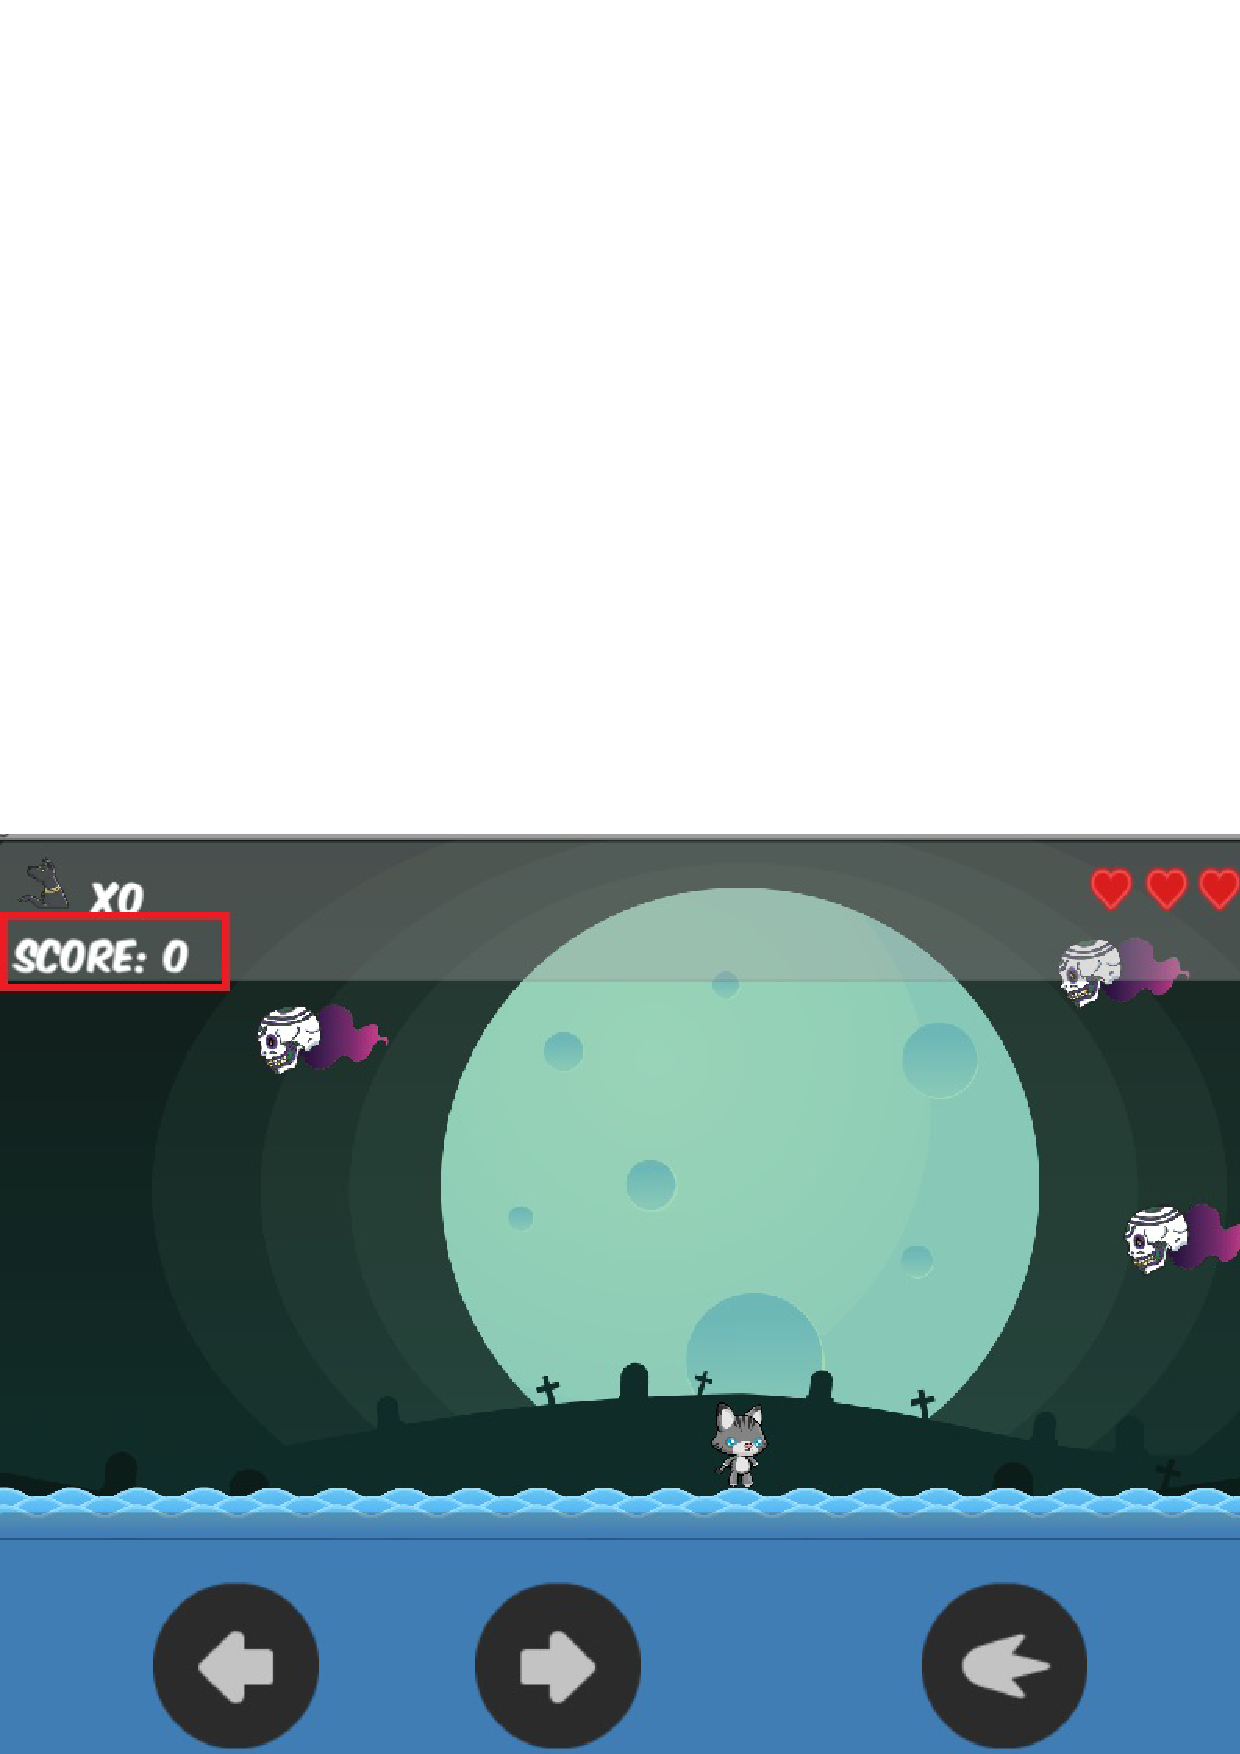
\includegraphics[width=0.4 \textwidth]{05TrabajoRealizado/03Unity/imagenes/02reaccionScore03}}
   
 	\subfigure[Actualización de marcador al derrotar a un enemigo (Autoría propia).] {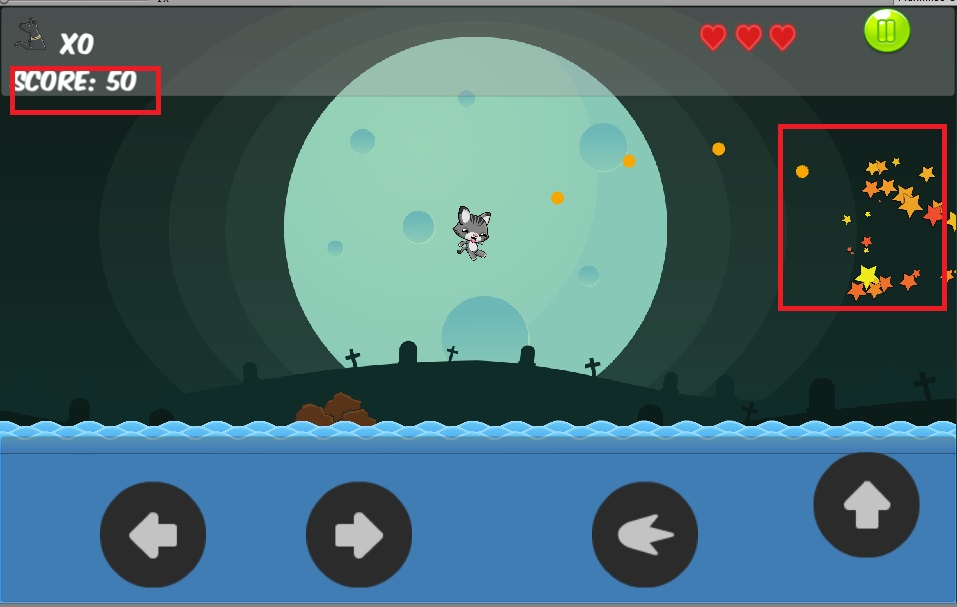
\includegraphics[width=0.4 \textwidth]{05TrabajoRealizado/03Unity/imagenes/02reaccionScore02}}

  \caption{Respuesta visual del juego cuando el personaje jugable derrota a un enemigo.}
  \label{figPersonajeResXo}
\end{figure}     
 
 \subsubsection{Patron de movimiento para los enemigos}
 Para la creación de los patrones de movimiento de los enemigos fue necesario  
 crear tres GameObjects vacíos para el enemigo de tipo PurpleGost(ver figura ) y dos 
 GameObjects vacíos para el enemigo de tipo RedGost. Utilizando la posición de los 
 GameObjects vacios cada tipo de enemigo sigue el patrón de movimiento desctrito en las 
 figura \ref{figPurpleGost} y \ref{figRedGost}.  

\begin{figure}
  \centering
   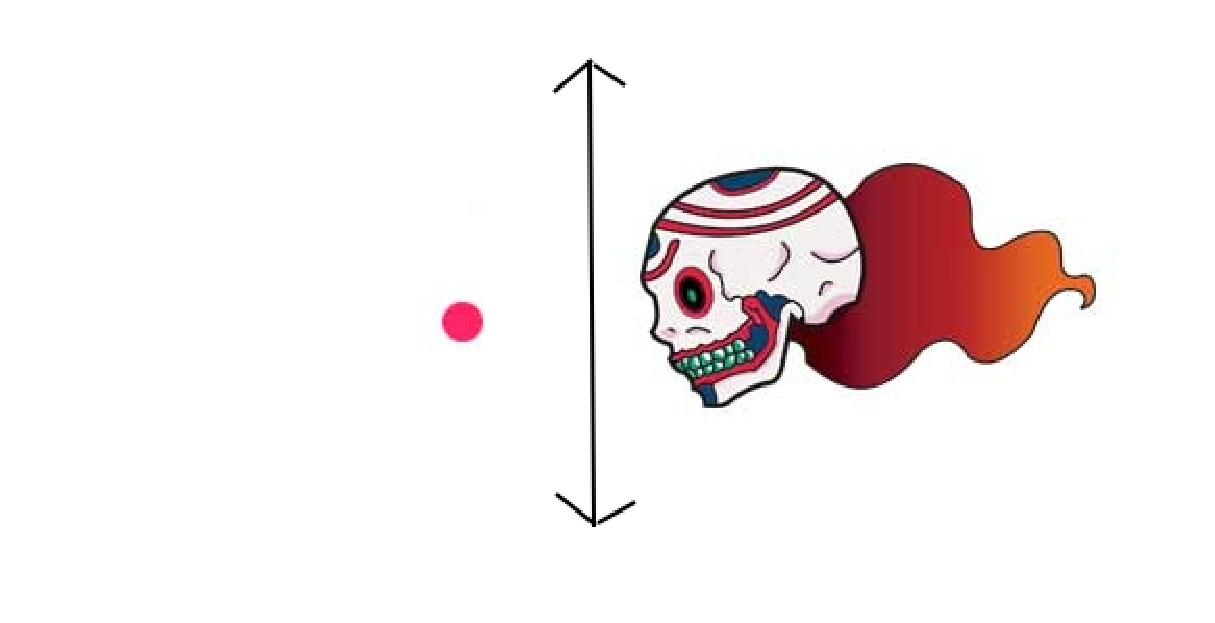
\includegraphics[width=0.4 \textwidth]{05TrabajoRealizado/03Unity/imagenes/disparoRojo}
  \caption{Patrón de movimiento de RedGost (Autoría propia)}
  \label{figRedGost}
\end{figure}

\begin{figure}
  \centering
   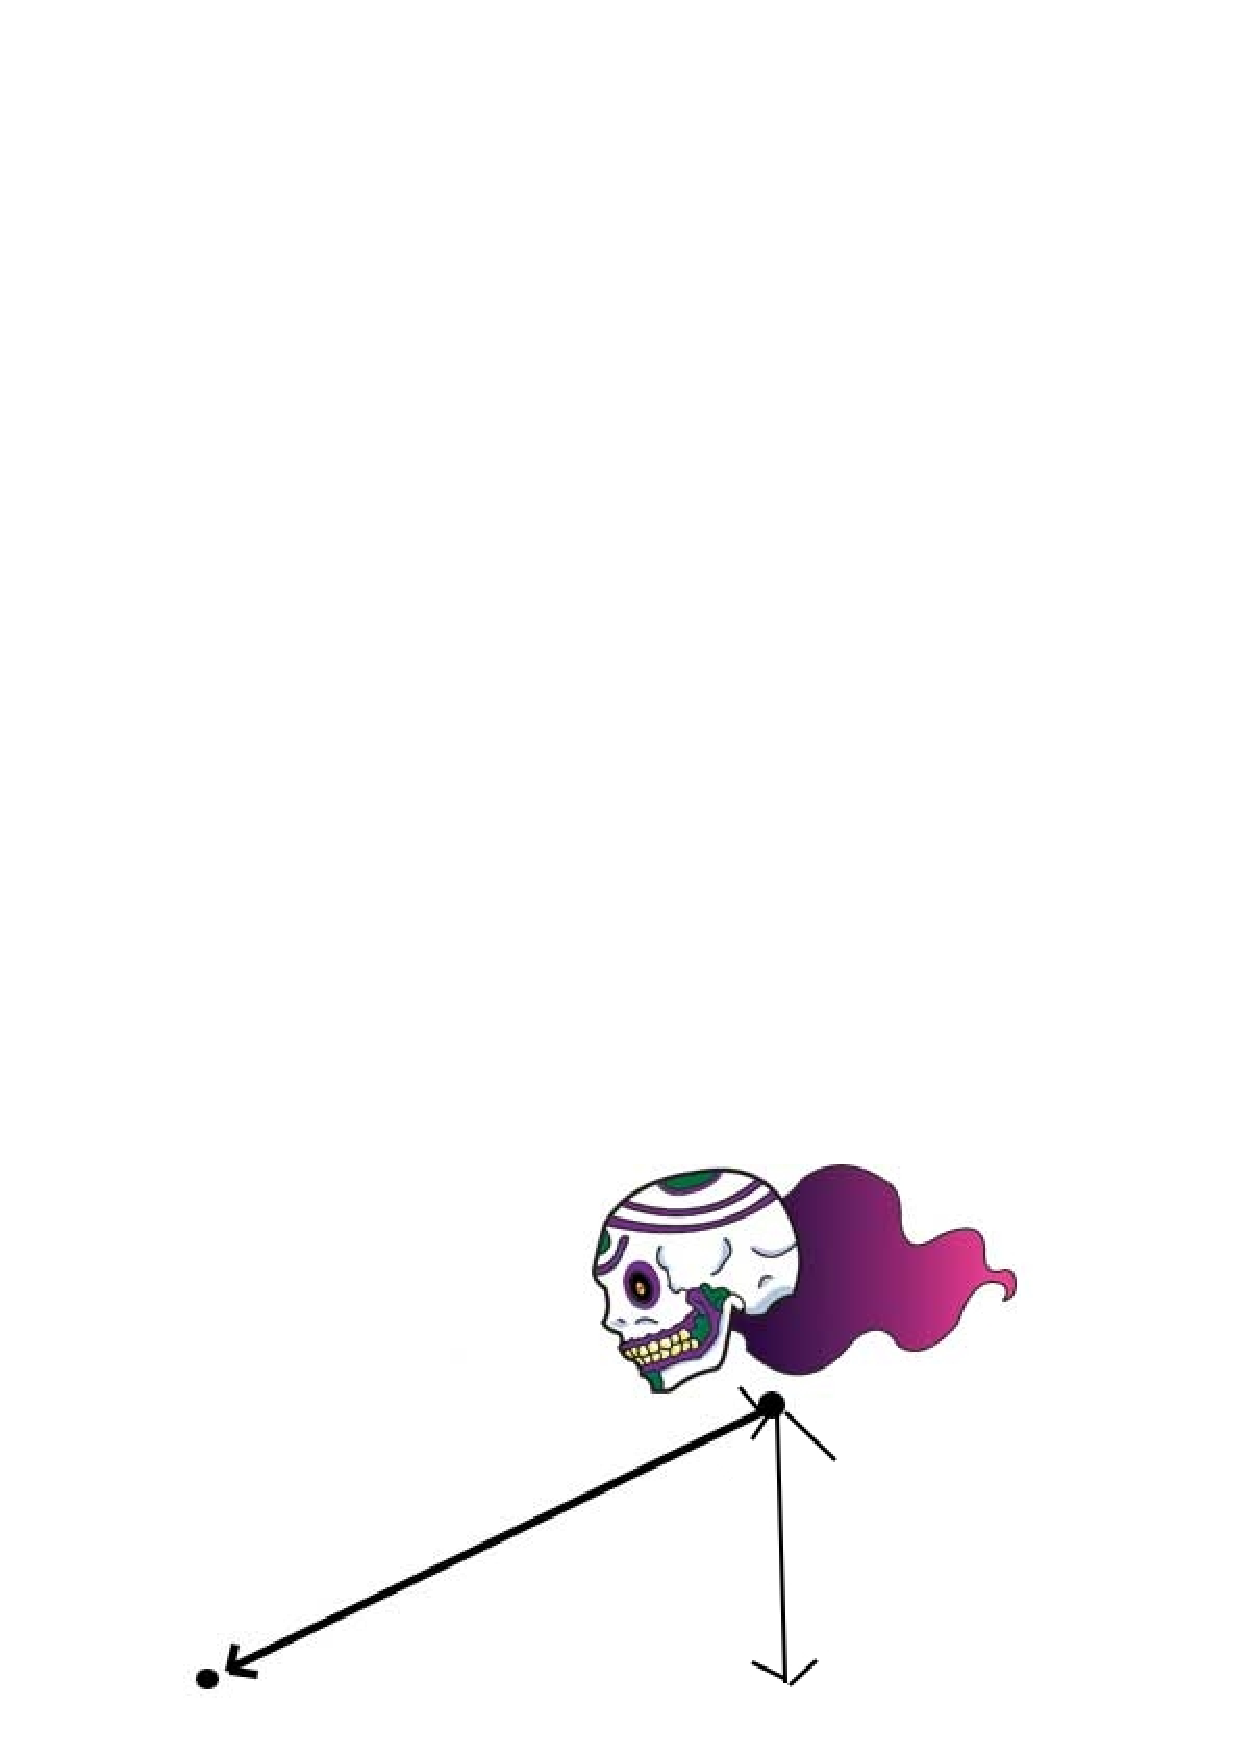
\includegraphics[width=0.4 \textwidth]{05TrabajoRealizado/03Unity/imagenes/embestida}
  \caption{Patrón de movimiento de PurpleGost (Autoría propia)}
  \label{figPurpleGost}
\end{figure}